\documentclass{article}
\usepackage{graphicx}
\usepackage{caption}
%\usepackage{minipage}
\usepackage{cmap}
\usepackage[russian]{babel}
\usepackage[utf8]{inputenc}
\begin{document}
\begin{center}
\large{Сравнение алгоритмов классификации на предмет устойчивости к зашумлению входных данных}
\end{center}
\newpage
\section{Постановка задачи}
Изобилие алгоритмов машинного обучения даёт определённый простор для выбора. К сожалению данные, предоставленные для обработки, зачастую содержат ошибки и неточности. Не секрет, что критериев такого сравнения можно придумать очень много, так почему бы не сравнить алгоритмы по устойчивости к порче входных данных? Для этого рассмотрим три популярных алгоритма: SVM, Decision Tree и Naive Bayes и рассмотрим их на датасете рукописных цифр, которые будем постепенно портить. Критерием качества работы алгоритма примем количество верно определенных цифр в тестовом множестве.
\section{Обзор предметной области}
\section{Практическая часть}
В качестве датасета был выбран MNIST Database, так как изображения в нём подвегнуты качественному перпроцессингу и мы можем быть уверены, что изображение испортили именно мы. Портить изображение будем наложением случайных шумов, как показано на рис.1.

\begin{figure}[h]
\centering
\begin{minipage}{.3\textwidth}
	\centering
	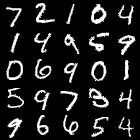
\includegraphics[width=\textwidth]{graphics/digits.jpg}
\end{minipage}
\begin{minipage}{.3\textwidth}
	\centering
	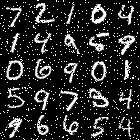
\includegraphics[width=\textwidth]{graphics/digits_spoiled10percent.jpg}
\end{minipage}
\begin{minipage}{.3\textwidth}
	\centering
	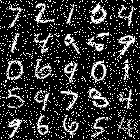
\includegraphics[width=\textwidth]{graphics/digits_spoiled20percent.jpg}
\end{minipage}
\caption{Пример зашумления изображений}
\end{figure}
Алгоритмы предполагается тестировать в двух ситуациях:
\begin{itemize}
\item Модель строится на незашумленных данных, а проверяется на испорченных
\item Модель строися и проверяется на зашумленных данных
\end{itemize}

\newpage
\section{Результаты}
График на рис.2 иллюстрирует зависимость корректности работы алгоритма от количества испорченных пикселей. Легко видеть, что эффективность Desicion Tree быстро падает и уже при 10\% испорченных пикселей количество корректных результатов падает до 50\%.
\begin{figure}[h]
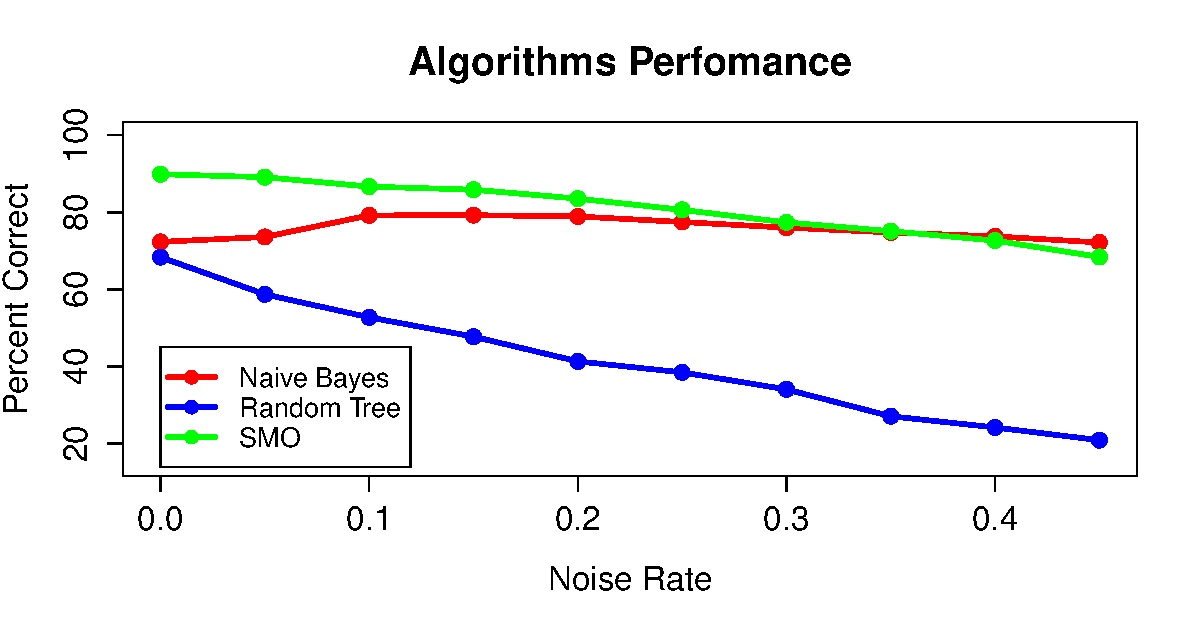
\includegraphics[width=\textwidth]{graphics/perfomance1.pdf}
\captionsetup{justification=centering}
\caption{Эффективность алгоритмов при построении модели на зашумленных данных}
\end{figure}
\end{document}